% Theoretische Grundlage, Berechnungsmethodik und Datensätze

\section{Theoretische Grundlagen und Datengrundlage}

In diesem Kapitel sollen die wichtigsten Grundlagen erläutert werden, um eine Bewertung des Einflusses der Nutzung des Speichersystems für die Erbringung von Primärregelleistung vornehmen zu können. Hierzu zählen die theoretischen Grundlagen der Erbringung von Primärregelleistung und des virtuellen Kraftwerks inklusive der verwendeten Hardware. Weiterhin wird auf die wichtigsten verwendeten Python und Matlab Befehle, sowie die verwendeten Datensätze und deren Aufarbeitung eingegangen. Zusätzlich wird das Vertragsmodell der sonnenFlat erläutert, um die Kostenstruktur darstellen zu können.

\subsection{Primärregelleistung}

Um zukünftig die Versorgungssicherheit gewährleisten zu können, müssen nicht nur erhebliche Mengen an Kraftwerksleistungen regenerativer Energieanlagen zugebaut werden, sondern auch die Erbringung von Systemdienstleistungen garantiert werden, welche bisher zum großen Teil durch konventionelle Großkraftwerke gedeckt werden. Ein wichtiger Baustein ist die Aufrechterhaltung der Netzfrequenz, welches durch die Erbringung von Regelleistung ermöglicht wird. Diese Simulation soll sich mit der Erbringung von Primärregelleistung befassen, welches die schnellste Art der Regelleistung im europäische Verbundsystem darstellt.\medskip\\
Der Zweck der Primärregelleistung liegt darin, die Netzfrequenz durch gezielte Leistungserbringung zu stabilisieren. Nötig wird dies, wenn eine Differenz zwischen dem Angebot und der Nachfrage an Leistung im Stromnetz besteht. Die Leistungserbringung wird automatisch durch eine Frequenzabweichung von der Soll-Netzfrequenz von \SI{50}{\hertz} aktiviert. Dabei wird durch die Übertragungsnetzbetreiber ein Totband von $\pm \SI{10}{\milli\hertz}$ definiert, in welchem keine Erbringung von Primärregelleistung erfolgen muss. Bei einer Abweichung von $\pm \SI{200}{\milli\hertz}$ muss hingegen die volle ausgeschriebene Regelleistung des Kraftwerks erbracht werden und dazwischen proportional zu der Frequenzabweichung \parencite{nextKW20}.


\subsection{sonnenBatterie eco 8.0}\label{sec:SB_eco8_Theorie}

Ein Schwarm aus Heimspeichern der sonnenBatterie eco 8.0 Serie bildet die physische Grundlage des virtuellen Kraftwerks. Bei der eco 8.0 handelt es sich um einen Lithium-Eisenphosphat-Akkumulator, dessen wesentlichen technischen Eigenschaften die Möglichkeiten des gesamten virtuellen Kraftwerks begrenzen.\\
Die einzelnen Batterien besitzen je nach Ausstattung eine nutzbare Batteriekapazität von \SIrange{4}{16}{\kwh}. Vereinfachend wird angenommen, dass nur sonnenBatterien mit einer Kapazität von mindestens \SI{8}{\kwh} eingesetzt werden. Ab einer Kapazität von  \SI{8}{\kwh} ist jede Batterie  mit einem Wechselrichter ausgestattet, der eine Nennleistung von \SI{3.3}{\kilo\watt} besitzt \parencite{sonnenBat18}.\\
Der mittlere Wirkungsgrad des Wechselrichters beträgt im Entladefall \SI{94.5}{\percent} und im Ladefall \SI{94.4}{\percent}. Weiterhin weißt die Batterie einen Wirkungsgrad von \SI{93.8}{\percent} auf \parencite{htwInspek19}.

\subsection{Das virtuelle Kraftwerk}\label{sec:VK_Theorie}

Das virtuelle Kraftwerk der Simulation wurde mit einer Gesamtleistung von \SI{1}{\mega\watt} präqualifiziert. Als Annahme wurden hierzu insgesamt 600 Heimspeicher der sonnenBatterie eco 8.0 Serie vernetzt, mit einer Gesamtleitung von \SI{1.98}{\mega\watt}. Der theoretische Leistungsspielraum des Kraftwerks liegt somit deutlich über der präqualifizierten Leistung.\\
Nötig ist dies aus verschiedenen Gründen. So kann beispielsweise nicht die Verfügbarkeit jeder Batterie zu jedem Zeitpunkt garantiert werden. Die einzelnen Batterien befinden sich in Privathand und unterliegen somit nur begrenzt der Kontrolle durch den Betreiber. Es kann zu Störungen der Hard- oder Software der einzelnen Batterien kommen, aber auch zu Störungen der Internetverbindung.\\
Die größten beschränkenden Faktoren des virtuellen Kraftwerks sind jedoch der Ladestand und der aktuelle Arbeitspunkt. Der Arbeitspunkt bestimmt, wie viel Regelleistung in positiver bzw. negativer Regelrichtung zur Verfügung steht. Als Regelleistung wird die Abweichung vom Arbeitspunkt verstanden. Der Arbeitspunkt der Batterien entspricht der eigenverbrauchsoptimierten Leistungsvorgabe.\\
Wenn der Ladestand zu gering bzw. zu hoch ist, kann die Erbringung der Regelleistung nicht in der gewünschten Dauer erfolgen. Bei einem zu hohen bzw. zu niedrigen Arbeitspunkt des Batteriepools kann das Kraftwerk bei einem Leistungsabruf nicht die geforderte Regelleistung erbringen. Durch aktives Lademanagement und das Einhalten von Grenzen für den Ladezustand muss im Realbetrieb die Erbringung der präqualifizierten Regelleistung garantiert werden.\\
Das grundlegende Funktionsprinzip des virtuellen Kraftwerks wird durch einen übergeordneten Regler bestimmt. Dieser wird in der Simulation stark vereinfacht. So wird von einem homogenen Verhalten der Batterien ausgegangen. Dies bedeutet, dass jede Batterie  die gleichen technischen Parameter besitzt und das sich die zugehörigen Photovoltaikanlagen ebenfalls identisch verhalten. Das führt dazu, dass den einzelnen Batterien feste Ladestandsgrenzen zugeordnet werden können, damit die Erbringung von Regelleitung im Bedarfsfall gewährleistet werden kann.

\begin{figure}[H]
	\begin{center}
		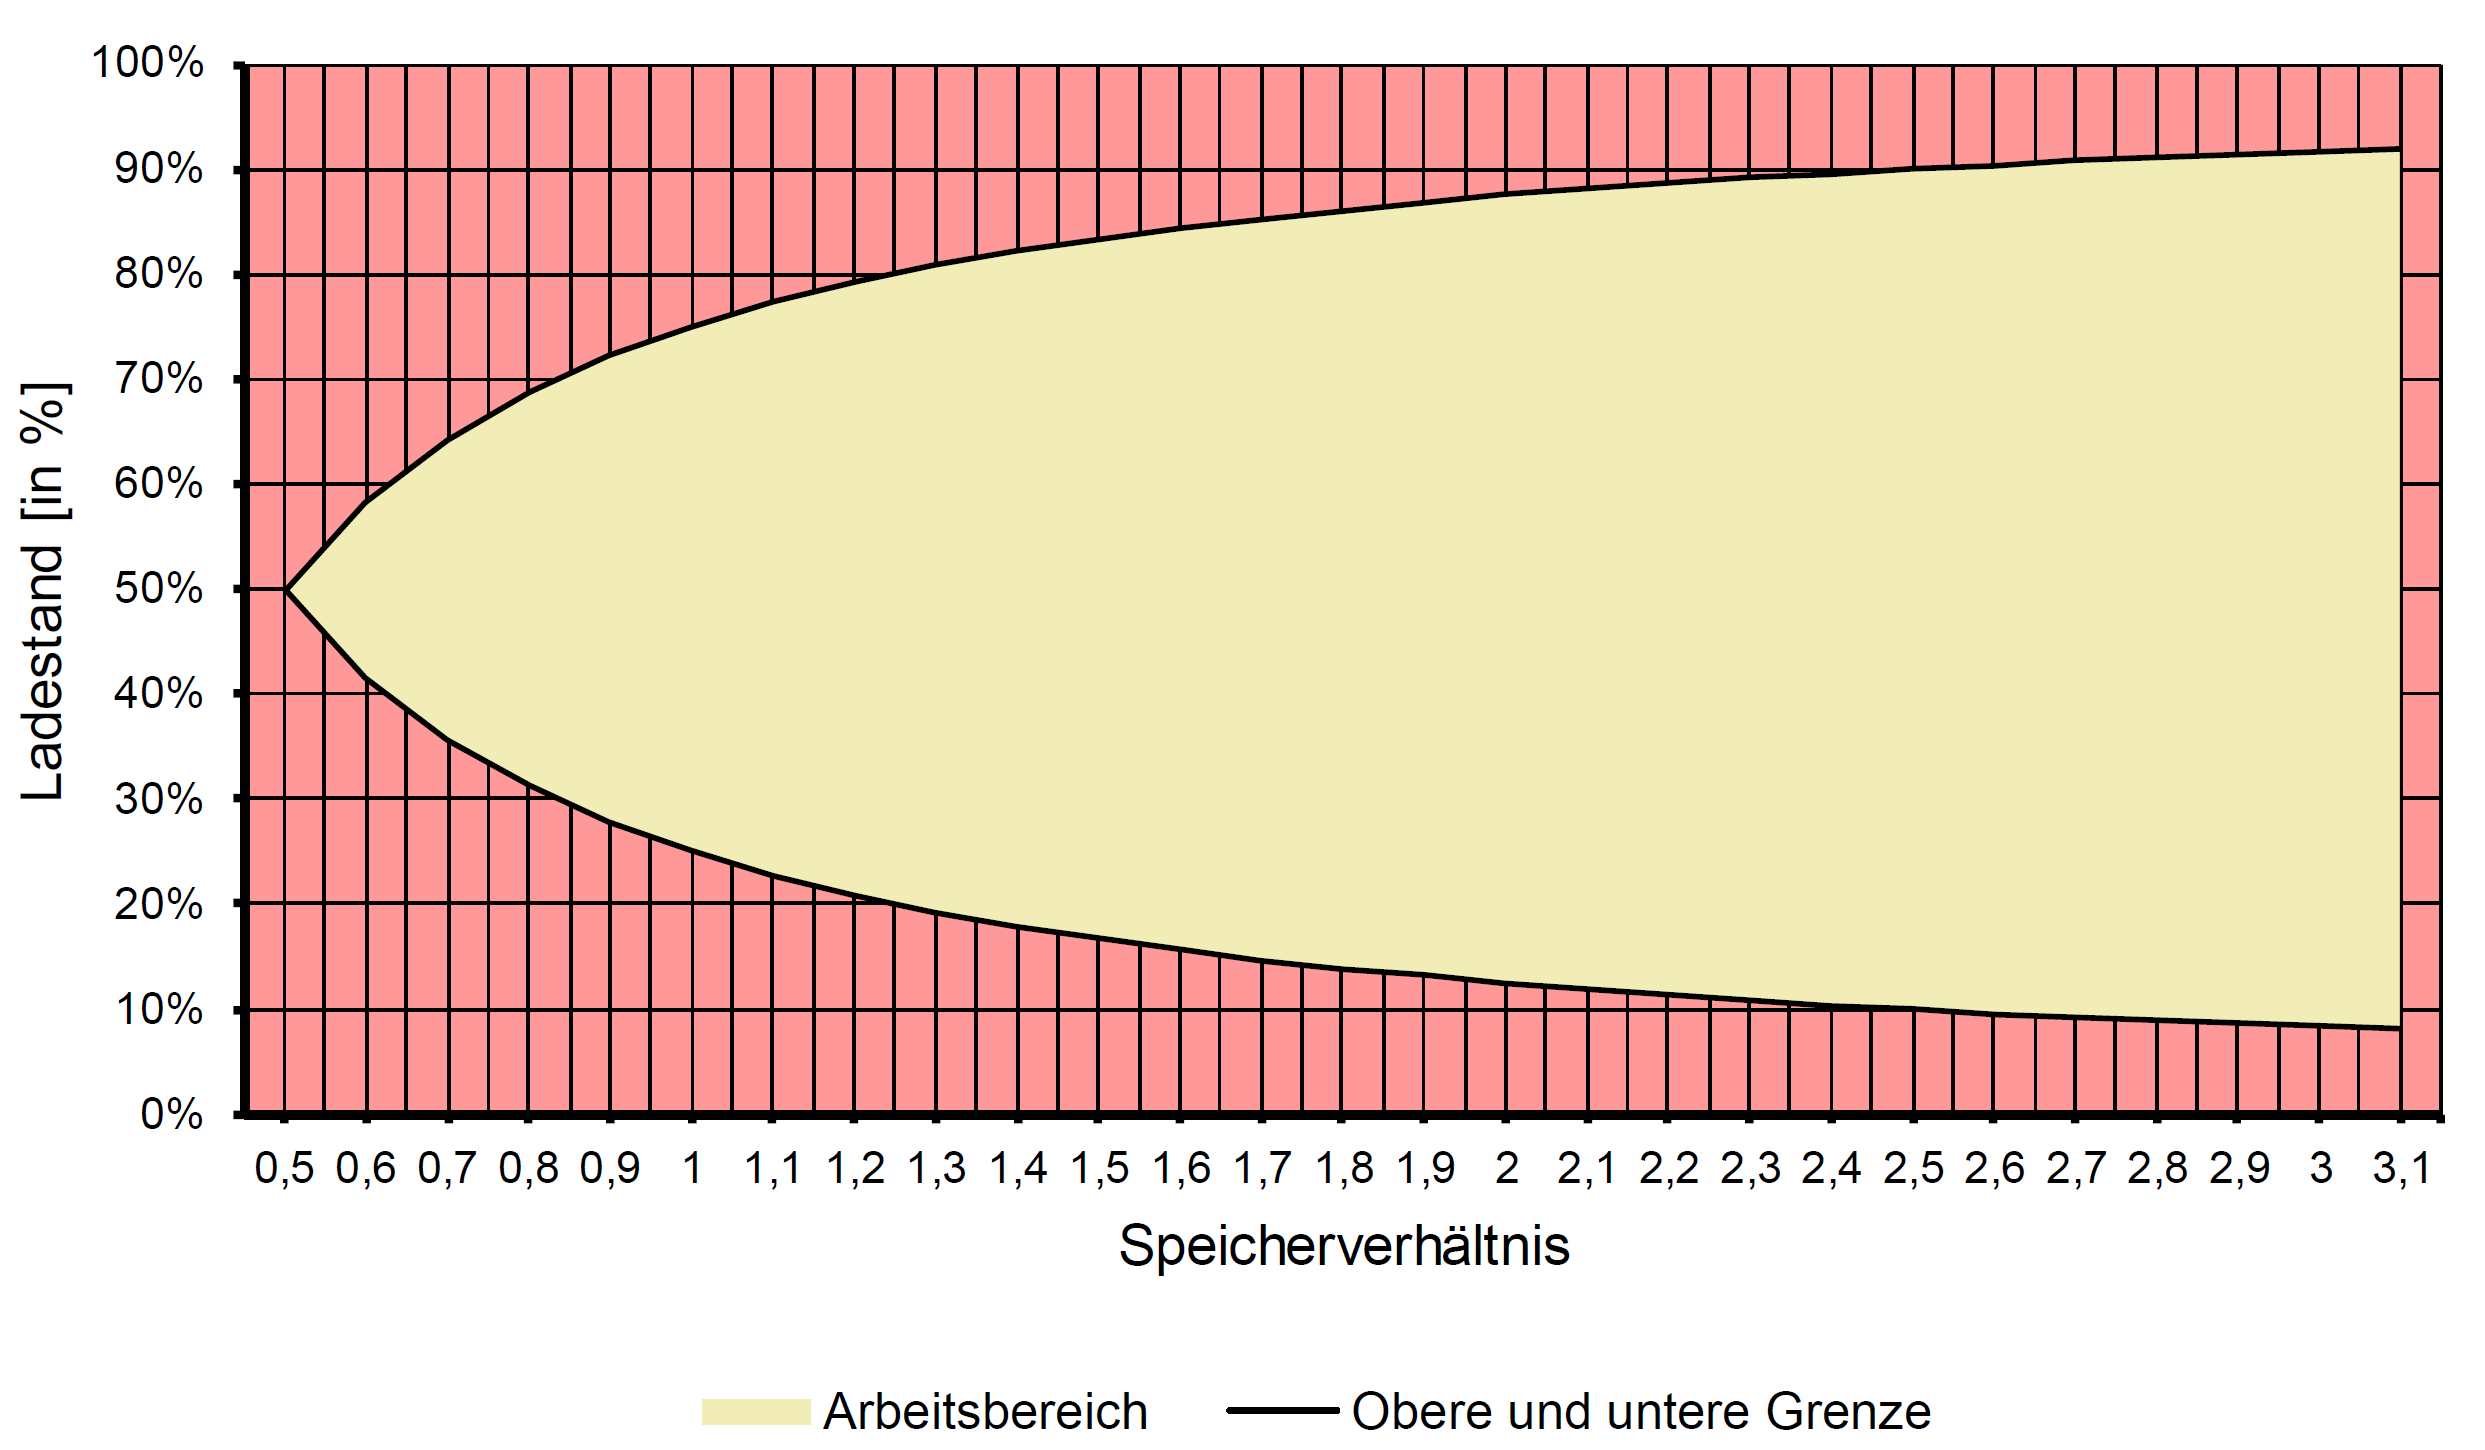
\includegraphics[width=\textwidth]{Bilder/P-E_factor.png}
		\caption{Zulässiger Arbeitsbereich bei der Erbringung von Primärregelleistung \parencite[s. S. 61][]{regel_PQ19}}
		\label{fig:P_E_factor}
	\end{center}
\end{figure}

\noindent Im Falle begrenzter Energiespeicher kommen die in Abbildung \ref{fig:P_E_factor} dargestellten zulässigen Arbeitsbereiche zur Anwendung. Durch dies wird sichergestellt, dass der Energiespeicher jederzeit seine vollständige angebotene Regelleistung für \SI{15}{\minute} zur Verfügung zu stellen.\medskip\\
In dem Fall des simulierten virtuellen Kraftwerks besteht ein Speicherverhältnis von \SIrange{4.8}{9.6}{}, je nach Größe der einzelnen Speichereinheiten. Da jedoch das Lademanagement innerhalb dieser Simulation nicht abgebildet werden kann, wurde sich für Ladestandsgrenzen von \SI{80}{\percent} im oberen und \SI{20}{\percent} im unteren Energiebereich entschieden.

\subsection{Die sonnenFlat}

Das Konzept der sonnenFlat beruht in erster Linie auf der sogenannten Freistrommenge. Diese dient als Leistungstausch für die Einschränkungen des eigenverbrauchsoptimierten Verhaltens der Batterie. Die Freistrommenge bezieht sich auf den Gesamtstromverbrauch und beinhaltet den Direktverbrauch der Photovoltaikanlage und den zusätzlichen Netzbezug. Der Netzbezug der Batterie für die Erbringung von Primärregelleistung wird getrennt bilanziert.

\begin{figure}[H]
	\begin{center}
		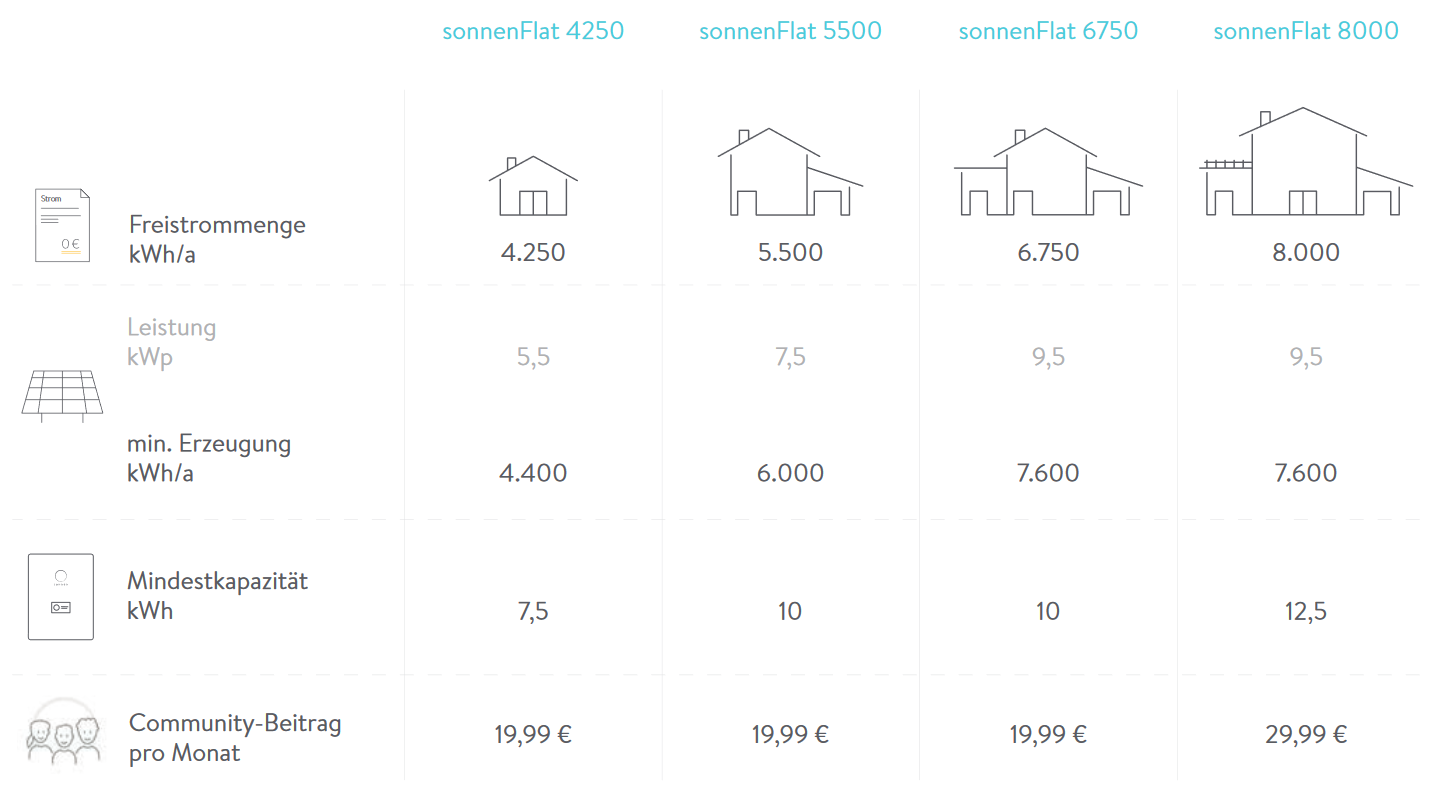
\includegraphics[width=\textwidth]{Bilder/flat.png}
		\caption{Varianten der sonnenFlat \parencite[s. S. 26][]{flat20}}
		\label{fig:flat_ver}
	\end{center}
\end{figure}

\noindent In Abbildung \ref{fig:flat_ver} sind die verschiedenen Varianten der sonnenFlat vorgegeben. Die Freistrommenge des Kunden hängt sowohl von der Leistung der Photovoltaikanlage und der Kapazität des Batteriespeichers ab. Die minimale Größe der Photovoltaikanlage beträgt hierbei \SI{5.5}{\kwp}, weshalb dies als minimale Größe der Simulation angenommen wurde. In dieser Simulation wird davon ausgegangen, dass der Kunde immer die für seine spezielle Situation größtmögliche sonnenFlat erhält. Hiervon ausgenommen ist die sonnenFlat 8000, da bei dieser höhere Community-Beiträge anfallen. Bei Überziehung der Freistrommenge von bis zu \SI{2000}{\kwh}, fallen bei der sonnenFlat Arbeitspreise von \SI{23}{\ctkwh} und darüber \SI{25.9}{\ctkwh} an \parencite{flat20}. Der Break-even-Point der sonnenFlat 8000 gegenüber der sonnenFlat 6750 ist somit ab einem jährlichen Stromverbrauch von \SI{7272}{\kwh} erreicht.\medskip\\
Eine weitere Besonderheit des sonnenFlat Vertrages ist der sogenannte sonnenBonus.. Hierbei handelt es sich um einen Aufschlag von  \SI{0.25}{\ctkwh} für jede eingespeiste Kilowattstunde der Photovoltaikanlage auf die übliche EEG-Vergütung \parencite{sonnenBonus20}.

\subsection{Verwendete Python und Matlab Befehle}

In diesem Kapitel werden die wichtigsten Python und Matlab Befehle erklärt. Auf Befehle, die bereits Teil der Vorlesung waren, wird nicht eingegangen.

\subsubsection*{Python}

\textbf{Glob}\\
Das \texttt{Glob}-Modul findet alle Pfadnamen, die mit einem angegebenen Muster übereinstimmen \parencite{PyGlob20}.\medskip\\

\noindent\textbf{Pandas}\\
\texttt{Pandas} bietet Funktionen für die Strukturierung und Analyse von Datensätzen \parencite{PyPan20}. Die wichtigsten verwendeten Befehle der \texttt{Pandas}-Bibliothek lauten wie folgt:

\begin{conditions}
	\text{\texttt{read\_csv()}}		&		Einlesen einer CSV-Datei als Datenfeld\\
	\text{\texttt{DataFrame()}}	&		Erstellt ein Datenfeld mit gewünschten Parametern\\
	\text{\texttt{multiply()}}		&		Ermöglicht Multiplikation eines Datenfeldes mit einem Skalar\\
	\text{\texttt{round()}}			&		Runden der Elemente eines Datenfeldes\\
	\text{\texttt{to\_csv()}}			&		Speichern eines Datenfeldes als CSV-Datei\\
	\text{\texttt{concat()}}			&		Verketten von einzelnen Datenfeldern\\
\end{conditions}


\subsubsection*{Matlab}

\textbf{Polyval}\\
Der Befehl \texttt{polyval(p, x)} wertet ein Polynom \texttt{p} an jedem Punkt in \texttt{x} aus. Das Argument \texttt{p} ist ein Vektor der Länge \texttt{n $+$ 1}, dessen Elemente die Koeffizienten (in absteigenden Potenzen) eines Polynoms \texttt{n}-ten Grades sind \parencite{MatPol20}:

\[ p\left(x\right)	= p_1 \cdot x^n + p_2 \cdot x^{n-1} + ... + p_n \cdot x + p_{n+1}	\]

\noindent\textbf{Reshape}\\
\texttt{Reshape} formt ein gegebenes Array in eine gewünschte Form um. Beispielsweise formt \texttt{reshape(A, [2,3])} \texttt{A} in eine 2-mal-3-Matrix um \parencite{MatRe20}.

\subsection{Datengrundlage}

Für die Simulation des Einflusses des virtuellen Kraftwerks kamen drei Datensätze zum Einsatz. Hierzu zählt ein Haushaltslastprofil, das Erzeugungsprofil einer Photovoltaikanlage und das Profil der Netzfrequenz im europäische Verbundsystem, welche modellexogen die Grundlage der Simulation bilden. Jeder Datensatz hat eine 1-minütige Auflösung und bildet ein ganzes Jahr ab. Die Aufarbeitung der einzelnen Datensätze erfolgt mit Hilfe von Python.

\subsubsection{Erzeugungsprofil der Photovoltaikanlage}

Das Erzeugungsprofil der Photvoltaikanlage wurde innerhalb der Vorlesung zur Verfügung gestellt. Dieses findet auch hier Anwendung und ist in der Datei \texttt{A04\_Daten.mat} hinterlegt. In der Variable \texttt{ppvs} ist die spezifische AC-Leistungsabgabe des Photovoltaik-Systems, normiert auf die nominale Photovoltaik-Generatorleistung hinterlegt.

\subsubsection{Haushaltslastprofil}

Das Haushaltslastprofil entspricht einem repräsentativen elektrische Lastprofile für Wohngebäude in Deutschland auf 1-minütiger Datenbasis. Dieses wird durch die Hochschule für Technik und Wirtschaft Berlin zur Verfügung gestellt \parencite{htwLast18}.\\
Verwendet wurde das dritte Lastprofil der Datei \texttt{CSV\_74\_Loadprofiles\_1min\_W\_var(1).zip}. Auch dieses wurde normiert. Dafür wurde zuvor die maximale Leistungaufnahme des Systems bestimmt und mit dieser die spezifische Leistungsaufnahme des Systems zu jeder Minute ermittelt.\medskip\\
Realisiert wurde dies mit folgendem Code:

\begin{code}
\captionof{listing}{Aufbereitung des Datensatzes des repräsentativen elektrischen Lastprofils für Wohngebäude}
\label{code:household}
\begin{minted}{python}
import pandas as pd

# Namen für die Spalten des Datensatzes bestimmen
names = list()
for i in range(74):
    names.append('H{}' .format(i+1))
    
# Einlesen der Daten
df_Load1 = pd.read_csv('DataRaw\\PL1.csv', names=names, sep=',')

# Ziel Datensatz isolieren und normieren
df_Household = pd.DataFrame()
df_Household['P_H'] = df_Load1.H3.multiply(1/max(df_Load1.H3))

# Speichern als .csv und runden
df_Household.round(5).to_csv('P_H.csv')
\end{minted}
\end{code}

\subsubsection{Profil der Netzfrequenz}

Das Profil der Netzfrequenz im europäische Verbundsystem liegt in 1-sekündiger Auflösung monatsweise für das Jahr 2018 vor. Zur Verfügung gestellt wurden die entsprechenden Datensätze durch Herrn Dipl.-Ing. (FH) Markus Jaschinsky \parencite{Jaschinsky18}.\medskip\\
Ziel der Aufarbeitung war es die einzelnen Profile zusammenzuführen und in eine 1-minütige Auflösung umzuwandeln. Anschließend sollte aus diesem Profil der Lastgang des virtuellen Kraftwerks, normiert auf die ausgeschriebene Primärregelleistung, ermittelt werden. Dieses erfolgte auf Grundlage des folgenden Codes:

\begin{code}
\captionof{listing}{Aufbereitung der Datensätze des Profils der Netzfrequenz im europäische Verbundsystem}
\label{code:VPP}
\begin{minted}{python}
import glob
import pandas as pd

# Namen der einzelnen Datein ermitteln
lst_csv = glob.glob("2018\*.csv", recursive=True)
# Spaltennamen festlegen
names = ['fq', 'delete']

# Ergebnisliste vorinitialisieren
lst_df = [0]*len(lst_csv)
i = 0

# Einlesen der einzelnen Datensätze
for name in lst_csv:
    lst_df[i] = pd.read_csv(name, names=names, sep=';')
    lst_df[i].index.name = 'ts'
    lst_df[i] = lst_df[i].drop(['delete'], axis=1)
    i += 1
    
# Zusammenführen der Monatsdatensätze
df_fq18 = pd.DataFrame()

for n in range(len(lst_df)):
    df_fq18 = pd.concat([df_fq18, lst_df[n]], sort=False)
    
# Umwandeln in 1-minütige Auflösung
df_fq18_minutes = df_fq18.copy().iloc[::60, :]

# Umrechnen der Netzfrequenz
# in die Sollvorgabe der Leistungserbringung des VPP
df_fq18_minutes['p_VPP'] =
[0 if 49.99 < fq < 50.01 else (50 - fq)*10/2 for fq in df_fq18_minutes.fq]

# Speichern als .xlsx
df_fq18_minutes.round(3).to_excel('P_VPP.xlsx')
\end{minted}
\end{code}

\newpage